\documentclass[10pt,addpoints]{exam}
\usepackage[utf8]{inputenc}
\usepackage[spanish,es-noshorthands]{babel}
\usepackage{hyperref}
\usepackage{amsmath}
\usepackage{amsfonts}
\usepackage{amssymb}
\usepackage{graphicx}
\usepackage{tikz}
\usepackage{multicol}
\usepackage[papersize={6.5in,8.5in},width=5.5in,height=7.5in]{geometry}
%\printanswers
\begin{document}
\title{\begin{minipage}{.2\textwidth}
        
\includegraphics[height=1.75cm]{Images/logo-colegio.png}
       \end{minipage}
\begin{minipage}{.55\textwidth}
 \begin{center}
Prueba Icfes 2014\\Matemáticas $11^{\circ}$
\end{center}
\end{minipage}
\begin{minipage}{.2\textwidth}

\includegraphics[height=1.75cm]{Images/logo-sed.png} 
\end{minipage}
}
\author{Germ\'{a}n Avendaño Ram\'{i}rez\\Lic. Matemáticas U.D., M.Sc. U.N.}
\date{}
\maketitle
\begin{center}
\fbox{\fbox{\parbox{5.5in}{\centering
Conteste en el cuadro de respuestas diseñado para tal fin.}}}
\end{center}
\vspace{0.1in}
\makebox[\textwidth]{Nombres: \hrulefill, curso:\underline{\hspace{48pt}}, fecha:\underline{\hspace{3cm}}}
\begin{questions}
\question
Una prueba atlética tiene un récord mundial de 10,49 segundos y un récord olímpico de 10,50
segundos. ¿Es posible que un atleta registre un tiempo, en el mismo tipo de prueba, que rompa
el récord olímpico pero no el mundial?
\begin{choices}
\CorrectChoice Sí, porque puede registrar, por ejemplo, un tiempo de 10,497 segundos, que está entre los dos tiempos récord.
\choice Sí, porque puede registrar un tiempo menor que 10,4 y marcaría un nuevo récord.
\choice No, porque no existe un registro posible entre los dos tiempos récord.
\choice No, porque cualquier registro menor que el récord olímpico va a ser menor que el récord mundial.
\end{choices}
\question En una institución educativa hay dos cursos en grado undécimo. El número de hombres y mujeres de cada curso se relaciona en la tabla:
{%
\newcommand{\mc}[3]{\multicolumn{#1}{#2}{#3}}
\begin{center}
\begin{tabular}{l|l|l|l|}\cline{2-4}
 & \mc{1}{c|}{\textbf{Curso 11A}} & \mc{1}{c|}{\textbf{Curso 11B}} & \mc{1}{c|}{\textbf{Total}}\\\hline
\mc{1}{|l|}{\textbf{Número de mujeres}} & 22 & 23 & 45\\\hline
\mc{1}{|l|}{\textbf{Número de hombres}} & 18 & 12 & 30\\\hline
\mc{1}{|l|}{\textbf{Total}} & 40 & 35 & 75\\\hline
\end{tabular}
\end{center}
}%
La probabilidad de escoger un estudiante de grado undécimo, de esta institución, que sea mujer es de $\frac{3}{5}$. Este valor corresponde a la razón entre el número total de mujeres y

\begin{choices}
 \CorrectChoice el número total de estudiantes de grado undécimo.
 \choice el número total de hombres de grado undécimo
 \choice el número total de mujeres del curso 11B.
 \choice el número total de hombres del curso 11A.
\end{choices}
%\question Para fijar un aviso público se coloca sobre un muro una escalera a 12 m del suelo (ver figura). Las figuras, además muestran la situación y alguna
\begin{minipage}{.5\textwidth}
\question En la tabla se presentan las cartas que conforman una baraja de póquer.\\

Si la probabilidad de escoger una de ellas que cumpla dos características determinadas es cero, estas características podrían ser:
\end{minipage}
\begin{minipage}{.5\textwidth}
\begin{center}
 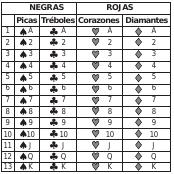
\includegraphics{./Images/baraja.jpg}
 % baraja.jpg: 0x0 pixel, 300dpi, 0.00x0.00 cm, bb=
\end{center} 
\end{minipage}
\begin{choices}
 \choice Ser una carta negra y ser un número par.
 \CorrectChoice Ser una carta roja y ser de picas
 \choice Ser una carta de corazones y ser un número impar.
 \choice Ser la carta roja K y ser de diamantes
\end{choices}
\question En una fábrica se aplica una encuesta a los empleados para saber el medio de transporte que usan para llegar al trabajo, y luego decidir si se implementa un servicio de ruta. Los resultados mostraron, entre otras, estas tres conclusiones sobre un grupo de 100 empleados que viven cerca de la fábrica y que se desplazan únicamente en bus o a pie:
\begin{itemize}
 \item El 60\% del grupo son mujeres
 \item El 20\% de las mujeres se desplazan en bus
 \item El 40\% de los hombres se desplaza caminando
\end{itemize}
¿Cuál de las siguientes tablas representa correctamente la información obtenida de ese grupo?
\begin{choices}
 \choice {%
\newcommand{\mc}[3]{\multicolumn{#1}{#2}{#3}}
\begin{tabular}{|l|l|l|}\hline
\mc{1}{|c|}{\textbf{Transporte/género}} & \mc{1}{c|}{\textbf{Hombre}} & \mc{1}{c|}{\textbf{Mujer}}\\\hline
En bus & 40 & 60\\\hline
Caminando & 60 & 40\\\hline
         \end{tabular}
}%
\CorrectChoice {%
\newcommand{\mc}[3]{\multicolumn{#1}{#2}{#3}}
\begin{tabular}{|l|l|l|}\hline
\mc{1}{|c|}{\textbf{Transporte/Género}} & \mc{1}{c|}{\textbf{Hombre}} & \mc{1}{c|}{\textbf{Mujer}}\\\hline
En bus & 34 & 12\\\hline
Caminando & 16 & 38\\\hline
               \end{tabular}
}%
\choice {%
\newcommand{\mc}[3]{\multicolumn{#1}{#2}{#3}}
\begin{tabular}{|l|l|l|}\hline
\mc{1}{|c|}{\textbf{Transporte/Género}} & \mc{1}{c|}{\textbf{Hombre}} & \mc{1}{c|}{\textbf{Mujer}}\\\hline
En bus & 0 & 20\\\hline
Caminando & 40 & 40\\\hline
               \end{tabular}
}%
\choice {%
\newcommand{\mc}[3]{\multicolumn{#1}{#2}{#3}}
\begin{tabular}{|l|l|l|}\hline
\mc{1}{|c|}{\textbf{Transporte/Género}} & \mc{1}{c|}{\textbf{Hombre}} & \mc{1}{c|}{\textbf{Mujer}}\\\hline
En bus & 24 & 12\\\hline
Caminando & 16 & 48\\\hline
               \end{tabular}
}%
\end{choices}
\question Se puede encontrar números racionales mayores que $k$, de manera que sean cada vez más cercanos a él, calculando $k+\frac{1}{j}$ (con $j$ entero positivo). Cuanto más grande sea $j$, más cercano a $k$ será el racional construído. ¿Cuántos números racionales se pueden construir cercanos a $k$ y menores que $k+\frac{1}{11}$
\begin{choices}
 \choice 10, que es la cantidad de racionales menores que 11
 \CorrectChoice Una cantidad infinita, pues existen infinitos números enteros mayores que 11.
 \choice 11, que es el número que equivale en este caso a $j$
 \choice Uno, pues el racional más cercano a $k$, se halla con $j=0$, es decir, con $k+0,1$
\end{choices}
\begin{minipage}{.55\textwidth}
\question El área de los rectángulos que se pueden construir a partir del origen, los ejes y un punto que pertenece a la gráfica de la función $f(x)=\frac{5}{x}$, donde $x>0$, se describe con la expresión $A_{x}=x\cdot f(x)$.
\end{minipage}\hfill
\begin{minipage}{.4\textwidth}
%Uncomment next line if XeTeX is used
%\def\pgfsysdriver{pgfsys-xetex.def}

\usetikzlibrary{arrows}
\baselineskip=10pt
\hsize=6.3truein
\vsize=8.7truein
\definecolor{zzttqq}{rgb}{0.6,0.2,0}
\definecolor{xdxdff}{rgb}{0.49,0.49,1}
\definecolor{uuuuuu}{rgb}{0.27,0.27,0.27}
\tikzpicture[line cap=round,scale=.5,line join=round,>=triangle 45,x=1.0cm,y=1.0cm]
\draw[->,color=black] (-0.62,0) -- (7.54,0);
\foreach \x in {,1,2,3,4,5,6,7}
\draw[shift={(\x,0)},color=black] (0pt,2pt) -- (0pt,-2pt) node[below] {$\x$};
\draw[->,color=black] (0,-0.56) -- (0,7.22);
\foreach \y in {,1,2,3,4,5,6,7}
\draw[shift={(0,\y)},color=black] (2pt,0pt) -- (-2pt,0pt) node[left] {$\y$};
\draw[color=black] (0pt,-10pt) node[right] {$0$};
\clip(-0.62,-0.56) rectangle (7.54,7.22);
\fill[color=zzttqq,fill=zzttqq,fill opacity=0.1] (0,0) -- (0,1.38) -- (3.72,1.34) -- (3.76,0) -- cycle;
\draw[line width=1.2pt, smooth,samples=100,domain=-0.6200000000000006:7.540000000000003] plot(\x,{5/(\x)});
\draw [color=zzttqq] (0,0)-- (0,1.38);
\draw [color=zzttqq] (0,1.38)-- (3.72,1.34);
\draw [color=zzttqq] (3.72,1.34)-- (3.76,0);
\draw [color=zzttqq] (3.76,0)-- (0,0);
\fill [color=uuuuuu] (0,0) circle (1.5pt);
\draw[color=uuuuuu] (0.16,0.26);
\fill [color=xdxdff] (0,1.38) circle (1.5pt);
\draw[color=xdxdff] (0.16,1.64);
\fill [color=xdxdff] (3.72,1.34) circle (1.5pt);
\draw[color=xdxdff] (3.88,1.6);
\fill [color=xdxdff] (3.76,0) circle (1.5pt);
\draw[color=xdxdff] (3.92,0.26);
\endtikzpicture 
\end{minipage}
\begin{multicols}{2}
 \begin{choices}
 \choice %Uncomment next line if XeTeX is used
%\def\pgfsysdriver{pgfsys-xetex.def}
\usetikzlibrary{arrows}
\baselineskip=10pt
\hsize=6.3truein
\vsize=8.7truein
\definecolor{uuuuuu}{rgb}{0.27,0.27,0.27}
\tikzpicture[line cap=round,scale=.5,line join=round,x=1.0cm,y=1.0cm]
\draw[->,color=black] (-0.8,0) -- (4.55,0);
\foreach \x in {,2,4}
\draw[shift={(\x,0)},color=black] (0pt,2pt) -- (0pt,-2pt) node[below] {$\x$};
\draw[->,color=black] (0,-0.51) -- (0,7.4);
\foreach \y in {,2,4,6}
\draw[shift={(0,\y)},color=black] (2pt,0pt) -- (-2pt,0pt) node[left] {$\y$};
\draw[color=black] (0pt,-10pt) node[right] {$0$};
\clip(-0.8,-0.51) rectangle (4.55,7.4);
\draw (0,0)-- (2.37,7.04);
\draw [color=uuuuuu] (0,0) circle (1.5pt);
\endtikzpicture
\CorrectChoice %Uncomment next line if XeTeX is used
%\def\pgfsysdriver{pgfsys-xetex.def}
\usetikzlibrary{arrows}
\baselineskip=10pt
\hsize=6.3truein
\vsize=8.7truein
\tikzpicture[line cap=round,line join=round,scale=.5,x=1.0cm,y=1.0cm]
\draw[->,color=black] (-0.26,0) -- (6.01,0);
\foreach \x in {,1,2,3,4,5,6}
\draw[shift={(\x,0)},color=black] (0pt,2pt) -- (0pt,-2pt) node[below] {$\x$};
\draw[->,color=black] (0,-0.3) -- (0,5.31);
\foreach \y in {,1,2,3,4,5}
\draw[shift={(0,\y)},color=black] (2pt,0pt) -- (-2pt,0pt) node[left] {$\y$};
\draw[color=black] (0pt,-10pt) node[right] {$0$};
\clip(-0.26,-0.3) rectangle (6.01,5.31);
\draw [line width=1.2pt] (0,5)-- (6,5);
\draw [color=black] (0,5) circle (1.5pt);
\endtikzpicture

\choice \tikzpicture[scale=0.5]
\draw[->] (-1,0) -- (4,0) node[right] {$x$};%Segmento de (-1,0) a (4,0)
\draw[->] (0,-1) -- (0, 4) node[left] {$y$};
% Dominio: domain = a:b?
\draw[smooth,domain=0.1:4,color=black]
plot (\x,{\x^2/4});
\draw (0,0) circle(2.5pt);
\endtikzpicture
\choice \tikzpicture[scale=0.5]
\draw[->] (-1,0) -- (5.2,0);%Segmento de (-1,0) a (4,0)
\foreach \x in {1,2,3,4}
\draw[shift={(\x,0)},color=black] (0pt,2pt) -- (0pt,-2pt) node[below] {$\x$};
\draw[->] (0,-.3) -- (0, 5.4) node[left] {$y$};
\foreach \y in {,1,2,3,4,5}
\draw[shift={(0,\y)},color=black] (2pt,0pt) -- (-2pt,0pt) node[left] {$\y$};
% Dominio: domain = a:b?
\draw[smooth,domain=.15:5,color=black]
plot (\x,{-\x^2/4+5});
\draw (0,5) circle(2.5pt);
\endtikzpicture
\end{choices}
\end{multicols}
\question Un colegio necesita enviar 5 estudiantes como representantes a un foro sobre la contaminación del medio ambiente. Se decidió que 2 estudiantes sean de grado décimo y 3 de grado undécimo. En décimo hay 5 estudiantes preparados para el foro y en undécimo hay 4. ¿Cuántos grupos diferentes pueden formarse para enviar al foro?

\begin{oneparchoices}
 \choice 9
 \choice 14
 \choice 20
 \CorrectChoice 40
\end{oneparchoices}
\question En determinada zona de una ciudad se construyen edificios de apartamentos en los que cada metro cuadrado tiene un costo de \$800\,000, y se asegura a los compradores que en esta zona anualmente, el metro cuadrado se valoriza un 5\% respecto al costo del año anterior. ¿Con cu\'al de las siguientes expresiones se representa el costo de un metro cuadrado en esa zona, transcurridos $n$ años?
\begin{multicols}{2}
 \begin{choices}
  \choice $800\,000+5n$
  \choice $800\,000(5n)$
  \choice $800\,000\left(\frac{5}{100}\right)^{n}$
  \CorrectChoice $800\,000\left(1+\frac{5}{100}\right)^{n}$
 \end{choices}
\end{multicols}
\question La expresión $10^{3}=\frac{I}{I_{0}}$ relaciona la sonoridad de un sonido de 30 decibeles con su intensidad $(I)$ y la menor intensidad $(I_{0})$ que percibe el oído humano.
¿Cuántas veces es el valor de $I$ respecto a $I_{0}$?

\begin{oneparchoices}
 \choice Una milésima
 \choice Un tercio
 \choice Tres veces
 \CorrectChoice Mil veces
\end{oneparchoices}
\question Entre los 16 estudiantes de un salón de clases se va a rifar una boleta para ingresar a un parque de diversiones. Cada estudiante debe escoger un número del 3 al 18. El sorteo se efectúa de la siguiente manera: se depositan 6 balotas en una urna, cada una numerada del 1 al 6; se extrae una balota, se mira el número y se vuelve a depositar en la urna. El experimento se repite dos veces más. La suma de los tres puntajes obtenidos determina el número ganador de la rifa. Si en la primera extracción del sorteo se obtuvo 2, es más probable que el estudiante que escogió el número 10 gane la rifa a que la gane el estudiante con el número 7, porque
\begin{choices}
 \choice al ser mayor  el número escogido, es mayor la probabilidad de ganar.
 \choice el primer estudiante tiene una posibilidad más de ganar que el segundo.
 \choice es más probable seguir obteniendo números pares.
 \CorrectChoice es mayor la diferencia entre 10 y 18 que entre 2 y 7.
\end{choices}
\question Un \emph{trapecio isósceles} es un cuadrilátero que tiene un solo par de lados paralelos y los otros dos, de igual medida.

En un plano cartesiano se dibuja un trapecio isósceles de modo que el eje $Y$ divide al trapecio en dos figuras iguales.

Si las coordenadas de dos de los vértices del trapecio son $(-4,2)$ y $(-2,8)$, ¿cuáles son las coordenadas de los otros dos vértices?
\begin{multicols}{2}
 \begin{choices}
  \choice (8,2) y (2,4)
  \CorrectChoice (2,8) y (4,2)
  \choice (--2,--4) y (--8,--2)
  \choice (--4,--2) y (--2,--8)
 \end{choices}
\end{multicols}
\question Los 70 empleados de una empresa están divididos en clase A y clase B. La empresa paga una prima de \$20\,000 a los empleados de clase A y de \$10\,000 pesos a los de clase B. Si el pago total de la prima es de \$1'200\,000, entonces el número total de empleados de clase A es

\begin{oneparchoices}
\choice 20
\choice 30
\choice 40
\CorrectChoice 50
\end{oneparchoices}
\question Al lanzar una vez un par de dados, la probabilidad de que salgan dos números consecutivos es:

 \begin{oneparchoices}
  \choice $\frac{10}{21}$
  \CorrectChoice $\frac{10}{36}$
  \choice $\frac{5}{21}$
  \choice $\frac{5}{36}$
 \end{oneparchoices}

%\answerline
\end{questions}
%cuadro de puntajes
%\begin{center}
%\gradetable[h][pages]
%\end{center}
\end{document}